\documentclass[pdflatex,sn-apa]{sn-jnl}% APA Reference Style
\usepackage{graphicx}%
\usepackage{multirow}%
\usepackage{amsmath,amssymb,amsfonts}%
\usepackage{amsthm}%
\usepackage{mathrsfs}%
\usepackage[title]{appendix}%
\usepackage{xcolor}%
\usepackage{textcomp}%
\usepackage{manyfoot}%
\usepackage{booktabs}%
\usepackage{algorithm}%
\usepackage{algorithmicx}%
\usepackage{algpseudocode}%
\usepackage{listings}%
\usepackage[normalem]{ulem}   % 支持 \sout 删除线
\usepackage{xcolor}           % 支持彩色文本
\usepackage[dvipsnames]{xcolor}
\usepackage{tikz}
\usetikzlibrary{arrows.meta, positioning}
%%%%
%% as per the requirement new theorem styles can be included as shown below
\theoremstyle{thmstyleone}%
\newtheorem{theorem}{Theorem}%  meant for continuous numbers
%%\newtheorem{theorem}{Theorem}[section]% meant for sectionwise numbers
%% optional argument [theorem] produces theorem numbering sequence instead of independent numbers for Proposition
\newtheorem{proposition}[theorem]{Proposition}% 
%%\newtheorem{proposition}{Proposition}% to get separate numbers for theorem and proposition etc.

\theoremstyle{thmstyletwo}%
\newtheorem{example}{Example}%
\newtheorem{remark}{Remark}%

\theoremstyle{thmstylethree}%
\newtheorem{definition}{Definition}%

\raggedbottom
%%\unnumbered% uncomment this for unnumbered level heads



\begin{document}

\title[Article Title]{Why Are Global P2P Lending Platforms Transforming Their Business Models? A Comparative Analysis of Risks and Regulations}


\abstract{In the past two decades, peer-to-peer (P2P) lending emerged as a disruptive innovation in financial intermediation, promising disintermediation, inclusivity, and efficiency. \sout{However, in recent years, a striking number of leading global P2P platforms—including Zopa, LendingClub, and Yiren Digital—have discontinued or significantly reduced their P2P lending operations, transitioning toward institutional funding models or digital banking structures.} \textcolor{NavyBlue}{However, in recent years, several leading global P2P platforms—including Zopa, LendingClub, and Yiren Digital—have discontinued or significantly reduced their P2P lending operations, transitioning toward institutional funding models or digital banking structures.} \sout{This study investigates the underlying causes of this widespread strategic retreat from P2P lending.} \textcolor{NavyBlue}{This study investigates the underlying dynamics driving this sector-wide shift away from original P2P intermediation models, examining how internal vulnerabilities and external institutional pressures have influenced strategic realignments among leading platforms.} Drawing on comparative analysis across eight prominent platforms in North America, Europe, and Asia, we trace platform evolution trajectories, identify shifts in product offerings, and examine changes in regulatory frameworks. Our findings suggest that two primary forces, internal risk pressures and escalating external regulatory constraints, have jointly driven the trend away from P2P lending. The analysis contributes to a deeper understanding of how innovation-led financial platforms evolve under institutional pressures, and raises broader questions about the sustainability of decentralized financial services in regulated environments.
}

%%================================%%
%% Sample for structured abstract %%
%%================================%%

% \abstract{\textbf{Purpose:} The abstract serves both as a general introduction to the topic and as a brief, non-technical summary of the main results and their implications. The abstract must not include subheadings (unless expressly permitted in the journal's Instructions to Authors), equations or citations. As a guide the abstract should not exceed 200 words. Most journals do not set a hard limit however authors are advised to check the author instructions for the journal they are submitting to.
% 
% \textbf{Methods:} The abstract serves both as a general introduction to the topic and as a brief, non-technical summary of the main results and their implications. The abstract must not include subheadings (unless expressly permitted in the journal's Instructions to Authors), equations or citations. As a guide the abstract should not exceed 200 words. Most journals do not set a hard limit however authors are advised to check the author instructions for the journal they are submitting to.
% 
% \textbf{Results:} The abstract serves both as a general introduction to the topic and as a brief, non-technical summary of the main results and their implications. The abstract must not include subheadings (unless expressly permitted in the journal's Instructions to Authors), equations or citations. As a guide the abstract should not exceed 200 words. Most journals do not set a hard limit however authors are advised to check the author instructions for the journal they are submitting to.
% 
% \textbf{Conclusion:} The abstract serves both as a general introduction to the topic and as a brief, non-technical summary of the main results and their implications. The abstract must not include subheadings (unless expressly permitted in the journal's Instructions to Authors), equations or citations. As a guide the abstract should not exceed 200 words. Most journals do not set a hard limit however authors are advised to check the author instructions for the journal they are submitting to.}

\keywords{Peer-to-Peer Lending, Platform Risk, Financial Regulation, FinTech Evolution}

%%\pacs[JEL Classification]{D8, H51}

%%\pacs[MSC Classification]{35A01, 65L10, 65L12, 65L20, 65L70}

\maketitle

\section{Introduction}\label{sec1}

Peer-to-peer (P2P) lending emerged in the early 2000s as an innovation in financial intermediation. It provided a digital alternative to traditional banking, allowing individuals to lend and borrow funds directly via online platforms without relying on financial institutions. The early appeal of P2P lending stemmed from its promise of disintermediation, reduced borrowing costs, higher investment returns, and expanded access to credit for underserved populations \citep{klafft_peer_2008, freedman_information_2017}. Platforms such as Zopa in the United Kingdom as well as LendingClub and Prosper in the United States became pioneers in this domain, rapidly gaining traction among retail borrowers and investors \citep{Morse2015463}. In subsequent years, the model expanded globally, with China becoming the largest P2P market by volume during the mid-2010s \citep{huang_online_2018}. This widespread adoption was supported by improvements in internet infrastructure, digital identity verification, and algorithmic credit scoring, which collectively enabled scalable and low-cost lending solutions \citep{bone-winkel_improving_2024}.

Despite its rapid global expansion and early optimism, the P2P lending industry has recently entered a period of profound contraction and structural transformation. \sout{A striking number of once-prominent P2P platforms have either permanently exited the P2P lending business or shifted their core models towards institutional funding or integrated banking services.} \textcolor{NavyBlue}{Several once-prominent P2P platforms have either permanently exited the peer-to-peer lending space or restructured their business models to prioritize institutional funding or integrated banking services.} Notable examples include Zopa, which surrendered its P2P license in 2021 and became a digital bank \citep{zopa_bank_limited_zopa_2021,zopa_bank_limited_our_2023}; LendingClub, which discontinued its retail P2P offerings after acquiring Radius Bank \citep{frankel_lendingclub_2020}; and Yiren Digital, which drastically restructured its consumer finance business in response to regulatory tightening in China \citep{economic_daily_p2p_2015, nemoto_optimal_2019}. Although these transitions differ in form, they collectively represent a broader retreat from the original P2P model that once emphasized peer-based credit risk sharing and decentralized loan funding.


\textcolor{NavyBlue}{These global developments raise a central research question: Why are P2P lending platforms across different jurisdictions transforming away from the original peer-to-peer model? To answer this question, this study adopts a comparative analytical approach to identify concrete drivers of the trend.} \sout{This paper explains the underlying causes of this global wave of platform exits from P2P lending, restructurings, or shifts in business orientation across jurisdictions.} This study adopts a comparative analytical approach to identify concrete drivers behind these decisions. We argue that two interrelated factors have played decisive roles: first, the persistent internal challenges associated with credit risk management; and second, the tightening of financial regulations, particularly those focused on enhancing investor protection, controlling systemic risk, and raising compliance standards \citep{ma_can_2022,shen_empirical_2021}. These forces have created a convergence of pressure that renders the original P2P lending model increasingly unsustainable both from an operational and economic point of view for major platforms operating at scale.

To investigate this phenomenon, we conduct a comparative analysis of eight representative P2P platforms across North America, Europe, and Asia. These include LendingClub, Prosper, Zopa, Funding Circle, Yiren Digital, Mintos, Bondora, and Faircent. Drawing on publicly available data, regulatory filings, and platform disclosures, we examine each platform's development trajectory, product evolution, and regulatory environment. Our aim is not only to describe platform-specific outcomes but to synthesize broader institutional and risk-based patterns that account for the observed strategic transformation from P2P lending. In doing so, this paper contributes to ongoing debates on the institutionalization of FinTech and the long-term sustainability of decentralized finance models under evolving regulatory regimes.

\textcolor{NavyBlue}{This study contributes to the literature on FinTech platform evolution in two important ways. First, it shifts the analytical focus from platform–user interactions to the institutional interface between P2P platforms and their regulatory environments, highlighting how business model adaptation emerges as a response to sustained institutional pressure. Second, it adopts a longitudinal and comparative perspective to trace platform-level transformations across jurisdictions and over time. This enables a dynamic understanding of how internal operational constraints and external rule changes jointly shape strategic transformation or structural transition. In doing so, the paper offers an integrated explanation for the decline of P2P lending models, contributing to broader debates on organizational adaptation in regulated financial ecosystems.}

\textcolor{NavyBlue}{
The remainder of this paper is organized as follows. Section~\ref{sec2} reviews the relevant literature on P2P lending, platform-based financial intermediation, systemic vulnerabilities, and platform governance. This section also clarifies the research gap and delineates the theoretical contributions of the study. Section~\ref{sec: methodology} describes the data sources, case selection rationale, and methodological approach. Section~\ref{sec: internal_factors} investigates the internal structures of major platforms by analyzing product offerings, business model shifts, and operational choices, thereby capturing platform-specific dynamics of strategic transition. Section~\ref{sec:external_factors} examines the external regulatory environment across jurisdictions, mapping policy shifts and compliance demands that have reshaped platform behavior. Together, these two empirical sections provide a comprehensive account of both internal and external pressures driving platform transformations. Section~\ref{sec:discussion} synthesizes the findings to highlight the interaction between internal constraints and regulatory tightening, discusses the fragmentation of the original P2P model, and outlines broader implications for platform governance and policy. Section~\ref{sec13} concludes.
}


\section{Related Work and Conceptual Background}\label{sec2}
\subsection{Literature on P2P lending evolution and risk exposure}\label{sec2.1}
P2P lending is a form of credit intermediation that enables individual borrowers to obtain loans directly from individual or institutional investors through an online platform \citep{eid_bridging_2024}. The typical lending process begins when a borrower submits a loan application, including basic financial and personal information. The platform then assesses the borrower's creditworthiness using proprietary risk models, which may incorporate credit scores, income data, and behavioral metrics \citep{liu_leveraging_2024}. Based on various mechanism, the platform determines the interest rate and loan terms \citep{zhou_bilateral_2019,shen_empirical_2021}, and either lists the loan request in a marketplace or directly matches it with lenders. After funding, the platform services the loan, collecting repayments or handling defaults.

P2P lending differs from traditional bank lending in several key aspects. First, banks typically perform due diligence using detailed, sometimes privileged information from the applicant's full financial history and transactional data. In contrast, P2P platforms rely on limited and often self-reported borrower information, supplemented by third-party credit data where available. Second, while banks maintain loans on their balance sheets and assume the associated credit risk, P2P platforms operate under an "originate-to-distribute" model, where risk is borne by the investors rather than the platform itself \citep{freedman_information_2017, lin_judging_2013}. Third, banks profit from the interest rate spread between deposits and loans, whereas P2P platforms generate revenue mainly through loan origination and servicing fees, typically charged as a percentage of the loan amount or repayment volume.

\subsection{The economic logic of platform-based financial intermediation}
The emergence of platform-based financial intermediation, particularly in the form of P2P lending, has drawn increasing scholarly attention as an institutional response to both technological advances and the shortcomings of traditional banking systems. From the perspective of financial intermediation theory, these platforms can be understood as novel arrangements for matching borrowers and lenders without relying on deposit-taking institutions. While traditional banks combine loan origination with credit and maturity transformation, P2P platforms primarily fulfill a brokerage role, facilitating credit allocation without assuming direct exposure to credit risk \citep{Havrylchyk2018115, Dömötör2021391}.

Several theoretical models have sought to explain the viability and appeal of P2P platforms relative to bank lending. For instance, \cite{Ben-Yashar2024939} develop a decision-theoretic model comparing the loan approval processes of banks and P2P platforms, showing that under certain conditions, such as less stringent regulation and distributed lending decisions, P2P platforms may extend credit more readily to risky borrowers. This supports the notion that P2P lending can complement bank credit in periods of procyclical credit contraction. Moreover, the platform model is often interpreted through the lens of multi-sided market theory, where platforms serve as intermediaries that reduce search costs, aggregate dispersed information, and coordinate matching across heterogeneous participants \citep{Berger200939}. These efficiencies are particularly relevant in environments where banks withdraw from marginal or subprime lending segments, as observed in the aftermath of the 2008 financial crisis \citep{Bavoso2020395}. In this context, P2P lending has been theorized as a form of market-based finance capable of enhancing financial inclusion and credit access for underserved borrowers. Technological innovations in data processing and credit scoring have further reinforced the logic of disintermediated lending. \cite{Georgiev2024587} argues that FinTech platforms exploit economies of scale in information collection and leverage both financial and non-financial data to reduce frictions in credit allocation. This supports the view that platform-based intermediation may partially replicate, or even improve upon, the screening functions traditionally performed by banks.

Nevertheless, despite their economic rationale, such platforms do not engage in liquidity or risk transformation, which limits their capacity to stabilize credit over time \citep{Havrylchyk2018115}. This inherent limitation distinguishes them from banks and raises questions about the resilience of the platform model in the face of systemic stress or borrower defaults. As a result, platform intermediation represents a new and distinct institutional form, justified by market imperfections and technological progress, yet structurally constrained in its scope and function.

\subsection{Systemic vulnerabilities of P2P lending}
Beyond the micro-level risk allocation discussed in Section \ref{sec2.1}, which primarily concerns the voluntary assumption of credit risk by individual lenders, a growing body of literature has drawn attention to the macro-level vulnerabilities embedded in platform-based lending. These systemic concerns are not directly linked to individual defaults, but arise from the structural features of platforms, including their network topology, lack of prudential regulation, and reliance on public trust, that may generate economy-wide consequences in times of stress. For instance, \citet{Li2018118} and \citet{Lu2018} apply network analysis to Chinese P2P markets and demonstrate how lending networks exhibit centrality concentration and path dependence, making some platforms systemically important due to their position within borrower-lender flows. Such configurations, according to these studies, increase the likelihood of contagion effects if major nodes fail. At the market level, \citet{Li20222596} employs conditional value-at-risk models to show how aggregate platform distress correlates with industry-wide capital flight and diminished liquidity, especially in times of elevated borrower default risk. These findings suggest that platform risk is not merely additive across loans, but may be amplificatory and self-reinforcing at the industry level. Moreover, \citet{Bavoso2020395} emphasizes that longer intermediation chains, such as those introduced by P2P securitization, introduce further opacity, undermining the original rationale of transparency and disintermediation that once legitimized P2P finance. 

Several studies further highlight how platform-based lending can generate reputational spillovers and information contagion, especially in the absence of formal institutional backstops. \citet{Cheng2022} uses the Ezubao scandal as a natural experiment to show that fraudulent platform failure significantly reduces borrower and investor activity on unrelated platforms, indicating that public trust operates at the sectoral rather than firm level. Similarly, \citet{Chen2021} argues that the eventual regulatory shutdown of China’s entire P2P sector reflected a broader loss of confidence in the platform model, rather than isolated misconduct. These authors point to the risks of transactional ambiguity and legal fluidity in markets where innovation outpaces regulation. In light of these dynamics, researchers such as \citet{Wei20161} and \citet{Thakor2020} suggest that platform intermediation, despite its technological form, shares functional similarities with traditional banking and should be subject to corresponding macroprudential oversight. Taken together, this literature indicates that platform-based lending may entail systemic vulnerabilities not despite its decentralized architecture, but precisely because of it, through structural fragility, risk concentration, and sector-wide interdependence.

\subsection{Platform governance and institutional adaptation}

\textcolor{NavyBlue}{Platform governance generally refers to the set of internal rules and mechanisms that platforms design to manage user behavior and coordinate multi-party interactions \citep{tiwana_chapter_2014}. Although this concept originated in the study of technology platforms, it has become increasingly relevant to financial intermediation platforms, especially in the P2P lending sector, where platforms not only match borrowers and lenders but also impose participation rules, risk controls, and disclosure standards.}

\textcolor{NavyBlue}{Recent empirical studies illustrate how various governance mechanisms affect FinTech platform performance and user behavior. For instance, \citet{Xia2023648} demonstrate that users’ institutional, technological, and interpersonal trust all influence their perceptions of platform governance, which in turn shapes their willingness to continue using FinTech services. Similarly, \citet{Chen20211055} show that the structural design and ownership configuration of P2P platforms—such as shareholder background, credit assignment mechanisms, and trusteeship—have measurable effects on net cash inflow and overall platform sustainability. These findings suggest that governance quality is not only a matter of internal architecture but also a determinant of platform viability in increasingly competitive and regulated markets. Moreover, several studies have moved beyond internal governance to examine how platforms adapt their strategies in response to shifting institutional environments. \citet{Wang2022}, for example, develop a tripartite evolutionary game model to analyze the co-governance dynamics among P2P platforms, investors, and regulators during the benign exit process in China’s lending sector, arguing that effective governance arises from the strategic alignment of incentives, penalties, and reputational constraints across stakeholders. Likewise, \citet{Lee20221} conceptualize data governance in the FinTech sector as a multilayered institutional architecture, involving both top-down regulatory frameworks and bottom-up compliance protocols enacted by platforms themselves. These perspectives underscore that platform governance in financial settings is not merely a matter of internal rule-making, but a continuous process of adjustment shaped by external institutional pressures and evolving norms.}

\textcolor{NavyBlue}{While these studies highlight the growing scholarly interest in how institutional environments shape platform governance, they often rely on theoretical models. This study examines how concrete regulatory changes and policy frameworks have influenced the governance structures of major P2P lending platforms across countries. By tracing platform responses to evolving market rules and supervisory mandates, the paper contributes an empirically grounded perspective to the discussion on governance adaptation in financial platforms.}

\subsection{Research gap and contribution of this study}

\sout{Although a growing body of literature has examined either the internal risk structures of P2P platforms or the external regulatory challenges posed by their emergence, few studies have integrated these two dimensions to explain the large-scale transformation of P2P lending in recent years.} \textcolor{NavyBlue}{While existing literature has examined P2P lending from multiple perspectives—including micro-level risk structures, the economic rationale of platform-based intermediation, and macro-level systemic vulnerabilities—most studies analyze these dimensions in isolation. Prior work typically treats platforms either as transactional mechanisms or as nodes of financial risk, but pays less attention to how P2P platforms adapt strategically over time in response to evolving regulatory and institutional pressures. As a result, current explanations for platform retreat or transformation often remain fragmented, overlooking the organizational dynamics that link internal constraints with external rule changes.}

\sout{This study addresses this gap by investigating why many prominent P2P platforms have closed or substantially reduced their P2P services. Rather than treating these outcomes as isolated business decisions, this paper interprets them as the result of interacting forces between platform-level vulnerabilities, such as credit risk management limitations and operational fragility, and the tightening of financial regulations aimed at preserving market integrity and protecting consumers. By tracing the trajectories of major platforms and linking them to institutional developments, this study offers an integrative and empirically grounded account of the decline of the P2P lending model.} \textcolor{NavyBlue}{This study addresses this gap by adopting a dynamic and comparative framework to examine platform retreat or transformation from P2P models across multiple jurisdictions. It makes two main contributions. First, it shifts analytical attention from platform–user interactions to the broader institutional interface between P2P platforms and regulatory systems. This reframing allows for a richer understanding of how platform strategies evolve under sustained compliance pressure and shifting supervisory regimes. Second, it offers a longitudinal analysis of platform evolution, tracing changes in product design, funding structure, and default risk management across time and context. This perspective moves beyond static typologies to show how platform outcomes are contingent on the sequencing and intensity of regulatory interventions.}




\section{Methodology}
\label{sec: methodology}
\subsection{Data sources}
The primary data sets for this study were collected from the official websites of eight major P2P lending platforms: LendingClub (\url{https://www.lendingclub.com/}), Prosper (\url{https://www.prosper.com/}), Zopa (\url{https://www.zopa.com/}), Funding Circle (\url{https://www.fundingcircle.com/}), Yiren Digital (\url{https://www.yirendai.com/}), Mintos (\url{https://www.mintos.com/}), Bondora (\url{https://www.bondora.com/}), and Faircent (\url{https://www.faircent.com/}). These platforms were selected based on their market relevance, international representativeness, and information availability. For each platform, relevant information concerning its founding background, business model evolution, operational trajectory, and market exit (where applicable) was systematically collected from public sources including official websites, annual and financial reports, platform-published disclosures, investor presentations, and archival screenshots where necessary. Given the limited availability of academic literature detailing platform-specific development histories, additional data were obtained from reputable financial news portals (Bloomberg, Financial Times, Caixin), industry white papers, regulatory announcements, and archival content preserved via web archives.

In addition to platform-level data, this study incorporates country-specific regulatory and policy information to contextualize platform operations within their respective institutional environments. Policy documents and legal texts were sourced from the official websites of national financial authorities, such as the Financial Conduct Authority (UK), the Securities and Exchange Commission (US), the European Securities and Markets Authority (Europe) and the China Banking and Insurance Regulatory Commission (China). If needed, secondary summaries from think tanks, legal databases, and expert commentary were used to supplement official documents and trace the evolution of key regulatory changes affecting the P2P lending sector. The integration of these regulatory sources enables an analysis of how external institutional factors interact with internal operational vulnerabilities to shape platform outcomes.

\subsection{Justification for platform selection}
The selection of these eight P2P lending platforms is justified by several key criteria:

\begin{enumerate}
    \item \textbf{Market leadership}: These platforms are recognized as leaders in their respective markets, either due to their large user bases, significant loan volumes, or innovative business models. For instance, LendingClub and Prosper are pioneers in the U.S. market, while Zopa holds the distinction of being the world’s first P2P lending platform \citep{bednorz_history_2023}.
    
    \item \textbf{Geographical diversity}: The platforms represent a diverse geographical spread, covering major P2P lending markets in North America, Europe, and Asia. This diversity allows for a comparative analysis of different regulatory environments, market dynamics, and platform trajectories.
    
    \item \textbf{Comprehensive services}: These platforms offer a wide range of financial products and services, from personal loans to business financing, and in some cases, auxiliary services such as investment management and credit scoring. 
    
    \item \textbf{Reputation and influence}: The selected platforms have established strong reputations and exert considerable influence on industry norms and investor expectations. Their developments often serve as bellwethers for the direction of the global P2P lending sector.
\end{enumerate}

\textcolor{NavyBlue}{
While the selected platforms provide meaningful coverage of major P2P markets and business models, we acknowledge certain limitations inherent in the sampling strategy. First, this study relies on publicly available data, which may not capture internal deliberations, informal regulatory interactions, or proprietary risk assessments that shaped strategic decisions. Second, the analysis focuses on relatively prominent and surviving platforms, excluding smaller or defunct platforms whose experiences might reveal additional patterns of fragility or failure. As such, our findings primarily reflect the trajectories of more resilient or visible actors in the industry. The conclusions drawn should therefore be understood as most applicable to platforms that have reached a certain scale or visibility and may not generalize to the broader population of smaller, short-lived, or regionally confined firms. Nevertheless, given the broad geographical scope, diversity of institutional contexts, and inclusion of both exited and transformed platforms, we believe the selected cases offer a representative basis for analyzing key drivers of platform evolution.}

\subsection{Research design and methodological approach}
This study adopts a qualitative, multiple-case comparative approach to investigate the institutional and operational dynamics underlying the retreat or transformation of major P2P lending platforms. Each platform is treated as a distinct case, situated within its respective regulatory and market context. The aim is to identify recurring patterns in internal business model vulnerabilities and the role of external interventions in shaping platform outcomes. Particular emphasis is placed on tracing the interaction between platform-level fragilities (e.g., risk management deficiencies, liquidity mismatches, scalability limits) and regulatory responses, including both formal legal enforcement and informal supervisory adjustments. Through cross-case comparison, the study uncovers shared causal mechanisms as well as divergences shaped by local institutional configurations. This design directly supports the study’s broader objective: to explain how the interplay of internal operational risks and external regulatory pressures drives platform exits, restructurings, or shifts in business orientation across jurisdictions.

\section{Business Model and Products: Internal Structures and their Role in Strategic Transition}
\label{sec: internal_factors}

To investigate the endogenous causes behind platform exits and strategic transitions in the P2P lending sector, we first examine the business model configurations and product structures adopted by major market participants. P2P platforms are approached not merely as service providers, but as institutional arrangements that embed specific operational logics, incentive structures, and risk-bearing mechanisms. By analyzing what platforms offer, how their products are structured, and how their loan and investment processes are organized, we uncover internal factors that may have contributed to their eventual retreat from or transformation within the P2P model.

To this end, we review the eight representative platforms along six key dimensions: 
\begin{itemize} 
\item What financial products does the platform offer? 
\item Does the platform allow loan applications? If so, who can apply for these loans (individuals, SMEs, institutions, etc.)? 
\item Does the platform allow investments? If so, who can invest (individuals, SMEs, institutions, etc.)? 
\item Is the platform still operating P2P lending products?  
\item If the platform is still operating P2P lending products, what is the business model? For instance, do investors directly choose borrowers, or does the platform allocate funds on their behalf? 
\item Who bears the default risk if the platform still operates P2P lending products? Is it the investors or the platform itself? 
\end{itemize}

These questions, though focused on operational features, provide the foundation for assessing each platform’s internal configuration. Following the descriptive review, we offer a brief analytical reflection for each case, identifying potential internal causes for the changes in the P2P lending structure. 

\subsection{Platform analysis}
\textbf{LendingClub} 
\begin{itemize} 
\item Financial products offered: LendingClub provides a variety of financial products including personal loans, auto refinancing, patient solutions loans, and small business loans. Additionally, LendingClub offers banking products such as high-yield savings accounts, checking accounts, and certificates of deposit (CDs). 
\item Loan Application: LendingClub allows individuals and small businesses to apply for loans. Borrowers can apply for personal loans ranging from \$1,000 to \$40,000, with terms of 2 to 5 years. Small business loans are also available, catering specifically to the financial needs of SMEs. 
\item Investment opportunities: LendingClub permits both individual and institutional investors to invest in loans. Historically, investors could purchase fractional shares of loans, known as “notes,” which represented portions of borrower loans. This allowed investors to diversify their investments across multiple loans to mitigate risk. However, it is important to note that LendingClub has transitioned its business model and no longer offers new “notes” as part of its investment opportunities. Currently, LendingClub focuses on whole loan sales to institutional investors, thus moving away from the traditional P2P lending model that initially allowed retail investors to fund loans directly. 
\item LendingClub no longer operates a traditional P2P lending model where individual investors directly fund loans to borrowers. This significant shift occurred after LendingClub acquired Radius Bank in 2021. The company has transitioned to a marketplace banking model, integrating traditional banking services with its lending platform. This change was driven by strategic business decisions to streamline operations and enhance financial stability. While the specific reasons for discontinuing the P2P model were not detailed extensively, it is clear that the transition allows LendingClub to leverage banking capabilities and offer a more comprehensive suite of financial products, catering primarily to institutional investors for loan funding. 
\item P2P lending model: Historically, LendingClub operated as a P2P platform where investors could directly choose which loans to fund. 
\item Default Risk: In LendingClub’s previous P2P model, the default risk was borne by the investors who purchased the notes. 
\end{itemize}

LendingClub’s decision to exit the traditional P2P model appears to reflect several internal considerations. In its early model, retail investors directly bore the default risk by purchasing fractional loan notes. While this allowed for portfolio diversification, it also relied heavily on investor trust in the platform’s underwriting and servicing. Over time, managing a large number of retail investors may have increased operational burdens. By acquiring a banking license and shifting to institutional loan sales, LendingClub moved toward a more stable and controllable funding model, suggesting that its original P2P structure had become difficult to sustain.

\vspace{1\baselineskip}
\textbf{Prosper}
\begin{itemize} 
\item Financial products offered: Prosper offers a range of financial products including personal loans, home equity loans (HELoans), home equity lines of credit (HELOCs), and credit cards. The platform allows borrowers to obtain personal loans ranging from \$2,000 to \$50,000, which can be used for various purposes such as debt consolidation, home improvement, and healthcare financing. Additionally, Prosper provides home equity products up to \$500,000 and credit cards with limits up to \$3,000.
\item Loan application: Prosper allows individuals to apply for loans. Borrowers can apply for personal loans as well as home equity products. The application process is designed to be quick, with the possibility of receiving funds as soon as the next business day after completing all necessary requirements.
\item Investment opportunities: Prosper permits individuals to invest in personal loans through its platform. Investors can purchase notes that correspond to portions of borrower loans, allowing them to diversify their investments across multiple loans. This investment opportunity is available to both individual and institutional investors, offering average historical returns of around 5.7\%.
\item Current status of P2P products: Prosper continues to operate as a P2P lending platform, allowing investors to fund personal loans directly. The platform has maintained its P2P model, enabling investors to choose loans based on their criteria, thus retaining the essence of P2P lending.
\item P2P lending model: Prosper operates on a model where investors can directly select the loans they wish to fund. Borrowers list their loan requirements, and investors can browse these listings to choose loans that match their investment preferences. This model provides transparency and control to investors in managing their portfolios.
\item Default risk: In Prosper’s P2P lending model, the default risk is borne by the investors who purchase the notes. While Prosper provides risk assessments and credit scoring to aid investment decisions, the ultimate risk of borrower default lies with the investors.
\end{itemize}

Compared to platforms that have exited the P2P model, Prosper has preserved its original disintermediated structure. Its product offering remains relatively focused on personal finance, and the platform continues to support direct matching between retail investors and borrowers. This suggests that Prosper has so far managed to align its operational model with its scale and market niche. The absence of banking integration or major structural overhaul indicates that Prosper has not experienced the same degree of internal misalignment or business model strain, at least not to the extent requiring transformation.

\vspace{1\baselineskip}
\textbf{Zopa}
\begin{itemize} 
\item Financial products offered: Zopa offers a range of financial products including personal loans, auto loans, credit cards, and savings accounts. The savings products include Smart Saver, Smart ISA, and Fixed Term Savings accounts. These products are designed to cater to various financial needs such as debt consolidation, home improvement, and general personal finance.
\item Loan application: Zopa allows individuals to apply for loans. The platform provides personal loans and car finance options. Borrowers can apply for these loans online, with the application process designed to be straightforward and user-friendly.
\item Investment opportunities: Zopa no longer offers traditional P2P investment opportunities. The platform closed its P2P lending business in January 2021 to focus on becoming a fully regulated digital bank. This decision was made to enhance regulatory compliance and operational efficiency, providing a broader range of financial services through Zopa Bank.
\item Current status of P2P products: As of now, Zopa does not operate any P2P lending products. The company transitioned away from the P2P model in 2021 to focus entirely on its banking operations and other financial services.
\item P2P lending model: Historically, Zopa operated a P2P lending model where investors could fund loans directly to borrowers. However, this model has been discontinued, and Zopa now functions solely as a digital bank.
\item Default risk: During its operation of the P2P model, the default risk was borne by the investors.
\end{itemize}

Zopa's withdrawal from the P2P lending space reflects a broader strategic transformation rather than a short-term operational response. As the first P2P platform globally, Zopa successfully scaled its retail investment model for over a decade, maintaining a relatively focused set of personal finance products. However, the shift toward digital banking suggests an internal reassessment of long-term viability. The decision to cease P2P services and pursue a banking license points to a desire for more stable funding sources and tighter control over compliance and capital adequacy. While Zopa did not publicly attribute this change to internal fragility, the move away from retail investor intermediation suggests challenges in sustaining the original marketplace model under growing operational and regulatory demands.

\vspace{1\baselineskip}
\textbf{Funding Circle}
    \begin{itemize}
        \item Financial products offered: Funding Circle provides a variety of financial products tailored to small businesses. These include business term loans, lines of credit, asset finance, and specialized loans under the Recovery Loan Scheme (RLS). Business loans range from £10,000 to £500,000 with terms up to 6 years, while lines of credit can range from £1,000 to £250,000. Asset finance options are available for funding vehicles, equipment, or machinery with loans up to £5 million.
        
        \item Loan application: Funding Circle allows SMEs to apply for loans. The platform specifically targets established small businesses, with criteria such as a minimum of two years in business and a minimum annual revenue of £50,000. Applicants must also meet certain credit requirements.
        
        \item Investment opportunities: Funding Circle permits both individual and institutional investors to invest in SME loans through its platform. Investors can diversify their investments across multiple loans to mitigate risk. The platform offers attractive returns by enabling investors to lend directly to small businesses.
        
        \item Current status of P2P products: Funding Circle continues to operate its P2P lending model, allowing investors to fund business loans directly. The platform has maintained its focus on P2P lending for small businesses, leveraging technology to facilitate these loans.
        
        \item P2P lending model: Funding Circle operates on a model where investors fund loans directly to small businesses. Investors can select loans based on their criteria, providing transparency and control over their investment choices. The platform also manages the loan servicing and collection processes.
        
        \item Default risk: In Funding Circle’s P2P lending model, the default risk is borne by the investors who lend money to businesses. While Funding Circle provides detailed credit assessments and risk ratings to aid investment decisions, the ultimate risk of borrower default remains with the investors.
    \end{itemize}

Funding Circle's business model remains rooted in SME-focused lending, with no publicly confirmed retreat from the P2P structure. Nonetheless, several features of its design reveal potential internal constraints. The platform targets a narrow borrower segment—established SMEs with minimum revenue thresholds—which may limit borrower volume and challenge scalability. Additionally, investors retain default risk, meaning that the platform must maintain robust credit assessments and servicing operations to preserve investor trust. While the platform still permits individual investment, the growing complexity of business loan underwriting and the platform’s expanding engagement with institutional capital suggest a potential shift toward more centralized funding mechanisms in the future. These features highlight Funding Circle’s efforts to balance transparency and operational control, while navigating the demands of a complex borrower segment.

\vspace{1\baselineskip}
\textbf{Yiren Digital}
    \begin{itemize}
        \item Financial products offered: Yiren Digital, also known as Yirendai, provides a range of financial products including personal loans, wealth management services, and insurance products. The platform primarily focuses on offering unsecured personal loans to meet various consumer needs such as home renovation, travel, and medical expenses. In addition, Yiren Digital has expanded its offerings to include wealth management products that cater to investors seeking diversified investment options.
        
        \item Loan application: Yiren Digital allows individuals to apply for personal loans. The platform targets high-growth potential individuals who may not have access to traditional banking services. The application process is facilitated online, leveraging big data and machine learning for credit risk assessment and loan approval.
        
        \item Investment opportunities: Yiren Digital offers investment opportunities primarily through its wealth management platform, where investors can choose from a variety of financial products designed to provide steady returns. However, specific details about the investment opportunities and whether they are available to individuals, small businesses, or institutions were not explicitly provided on the platform's website.
        
        \item Current status of P2P products: Yiren Digital continues to operate its P2P lending products. The platform maintains a focus on personal loans facilitated through advanced technology to ensure efficient loan matching and risk management.
        
        \item P2P lending model: Yiren Digital operates a P2P lending model where investors do not directly select borrowers. Instead, the platform uses an algorithm to match lenders with borrowers, optimizing the allocation of funds based on risk assessments and borrower profiles. This model ensures that the process remains efficient and scalable.
        
        \item Default risk: In Yiren Digital’s P2P lending model, the default risk is typically borne by the investors. The platform provides detailed credit assessments to help investors make informed decisions, but the ultimate risk of borrower default lies with the lenders.
    \end{itemize}

Yiren Digital’s operational structure reflects several features that may contribute to internal fragility. The platform relies on algorithmic matching to allocate funds between investors and borrowers, which helps streamline processes but limits transparency and control for lenders. Unlike traditional P2P models where investors actively select loans, this automated system reduces investor agency while preserving exposure to default risk. Additionally, the platform’s expansion into wealth management and insurance suggests a move to diversify income sources beyond lending, which may imply that the core lending business alone is insufficiently resilient or scalable. 

\vspace{1\baselineskip}
\textbf{Bondora}
    \begin{itemize}
        \item Financial products offered: Bondora provides a variety of financial products primarily focused on consumer loans and investment opportunities. The platform's flagship product is "Go \& Grow," an automated investment service that allows users to invest in loan portfolios with expected returns of up to 6.75\% per annum. Bondora also offers Portfolio Manager and Portfolio Pro, which enable investors to customize their investment strategies based on risk preferences and loan selection criteria.
        
        \item Loan application: Bondora allows individuals to apply for consumer loans. Borrowers can apply for personal loans directly through the platform, which offers a streamlined and quick loan approval process. The platform caters primarily to individual consumers, providing them with accessible credit options.
        
        \item Investment opportunities: Bondora offers several investment opportunities to individuals. Investors can choose from Go \& Grow, Portfolio Manager, and Portfolio Pro, each providing different levels of control and automation. These options are designed to cater to both novice investors looking for simplicity and experienced investors seeking more control over their portfolios.
        
        \item Current status of P2P products: Bondora continues to operate its P2P lending model, allowing investors to invest in loans issued to borrowers across Europe. The platform has maintained its P2P structure, with investments primarily funneled through the Go \& Grow product, which simplifies the investment process and provides automated portfolio management.
        
        \item P2P lending model: Bondora operates on a model where investors can choose to manually select loans via Portfolio Pro or automate their investments through Go \& Grow and Portfolio Manager. This model ensures a balanced approach, offering both direct loan selection and automated investment strategies for diversifying portfolios.
        
        \item Default risk: In Bondora’s P2P lending model, the default risk is borne by the investors. The platform provides detailed risk assessments and loan ratings to help investors make informed decisions. However, the ultimate risk of borrower default lies with the investors themselves, which is a common structure in P2P lending platforms.
    \end{itemize}

Bondora’s product design emphasizes investor convenience through automation, but this comes with reduced control over individual credit selection. The centrality of Go \& Grow in its investment structure reflects a shift toward simplicity and accessibility, particularly for retail investors. However, this model relies heavily on the platform’s internal risk assessment and portfolio allocation strategies, creating potential opacity in loan-level decision-making. Additionally, available data indicate a rising trend in default rates in recent years, suggesting that the long-term sustainability of the model may depend on the platform’s ability to adapt its underwriting practices and maintain portfolio quality under growing scale.

\vspace{1\baselineskip}
\textbf{Faircent}
    \begin{itemize}
        \item Financial products offered: Faircent offers a range of financial products primarily focused on P2P lending. These include personal loans and business loans. The platform connects borrowers and lenders directly, providing a virtual marketplace for loan transactions. Faircent also offers various investment plans for lenders, such as Fixed Term, Monthly Income, and On-Demand plans, which are designed to suit different investment needs and preferences.
        
        \item Loan application: Faircent allows individuals and businesses to apply for loans. Borrowers can apply for personal loans or business loans directly through the platform. The application process involves a comprehensive verification of the borrower’s personal, financial, and professional information to ensure creditworthiness and repayment capability.
        
        \item Investment opportunities: Faircent permits individuals to invest in loans. Investors can choose from different investment plans, allowing them to pool their money into a diverse mix of loans offered to pre-verified borrowers. The platform uses advanced data analytics to match lenders with creditworthy borrowers, providing a transparent and efficient investment process.
        
        \item Current status of P2P products: Faircent continues to operate its P2P lending model actively. The platform is regulated by the Reserve Bank of India (RBI) as an NBFC-P2P, ensuring compliance with financial regulations and maintaining its status as a leading P2P lending marketplace in India.
        
        \item P2P lending model: Faircent operates a P2P lending model where investors do not directly choose individual borrowers. Instead, the platform uses algorithms to match lenders with suitable borrowers based on various parameters. This approach helps streamline the lending process and ensures efficient allocation of funds.
        
        \item Default risk: In Faircent’s P2P lending model, the default risk is borne by the investors. The platform provides detailed assessments and continuous monitoring to help manage and mitigate risk, but the ultimate responsibility for potential defaults lies with the lenders themselves.
    \end{itemize}

Faircent’s model emphasizes automated credit matching and diversified loan pooling, which lowers the burden on individual investors to assess borrower risk manually. This strategy may improve efficiency and scalability but also reduces transparency in credit selection. The platform’s expansion into multiple investment plans and the absence of granular investor control point to a system increasingly reliant on internal algorithms and credit scoring mechanisms. While Faircent remains active in the Indian market under RBI regulation, its long-term sustainability will likely depend on the effectiveness of these algorithmic risk assessments in managing default exposure under varying economic conditions.

\subsection{Concluding Remarks on Internal Factors}
This section has examined the evolution and structural features of eight major P2P lending platforms, focusing on their business models, financial products, and operational configurations. Through a platform-by-platform analysis, several common patterns and divergences emerge regarding the internal factors that have shaped strategic transitions in the P2P sector.

First, product offerings and investment structures varied significantly across platforms, reflecting different market strategies and risk allocations. Some platforms, such as LendingClub and Zopa, initially adopted models centered on retail investors funding standardized consumer loans but eventually transitioned toward bank-based or institutional models. Others, like Prosper and Funding Circle, have continued to operate P2P structures, albeit with refinements in loan matching and investor engagement. These shifts suggest that the sustainability of the P2P model is closely linked to the platform’s ability to manage investor trust, credit performance, and product scalability.

Second, several platforms displayed signs of operational strain or model adaptation that point to underlying fragilities. For instance, complex loan servicing logistics, thin or opaque secondary markets, and the burden of maintaining regulatory compliance for retail investment products were recurring challenges that likely motivated business model reconfiguration. In some cases, such as Yiren Digital and Faircent, the introduction of algorithm-based loan allocation and institutional-style underwriting reflects a move toward tighter platform control over credit risk, albeit without formally abandoning P2P principles.

Taken together, these cases illustrate that internal operational considerations—including scalability, investor risk exposure, and cost-efficiency—play a pivotal role in shaping platform-level decisions to retain, transform, or exit the P2P model. While each platform’s trajectory is shaped by its specific market context and institutional constraints, the patterns suggest that endogenous pressures, rather than exogenous shocks alone, are central to understanding the decline or adaptation of P2P lending platforms.

\section{Regulatory Environment and External Pressures}
\label{sec:external_factors}
This section investigates the external institutional factors that have shaped the strategic choices of P2P lending platforms, with particular attention to regulatory frameworks and supervisory dynamics. As platforms scaled and attracted broader public and policy attention, regulatory scrutiny intensified, reshaping their operational boundaries and compliance obligations. By examining how P2P lending is regulated across different jurisdictions, and how specific regulatory changes influenced platform behavior, we aim to understand the extent to which external institutional pressures contributed to platform transformations or exits. Through this analysis, we assess how legal, supervisory, and policy environments constrained or enabled the sustainability of disintermediated lending models.

\subsection{LendingClub}

\textbf{Regulatory environment}

LendingClub has operated under an increasingly stringent regulatory framework since its inception. As a P2P lending platform, it was subject to both federal and state-level oversight, including registration of loan offerings as securities with the U.S. Securities and Exchange Commission (SEC) and compliance with investor protection and disclosure rules. This positioning required ongoing monitoring, standardized documentation, and investor risk disclosures.

A major regulatory shift occurred in 2021 when LendingClub acquired Radius Bancorp and became a regulated digital bank. This transformation brought the company under the authority of the Office of the Comptroller of the Currency (OCC) and the Federal Reserve. As a banking institution, LendingClub became subject to expanded compliance obligations, including capital adequacy requirements, anti-money laundering (AML) protocols, and the Community Reinvestment Act (CRA) (12 CFR Part 25).

\textbf{Regulatory changes and impact}

The shift to a banking model directly impacted LendingClub’s ability to sustain its original P2P lending framework. Compliance with bank-level regulatory standards increased the operational complexity of offering loan “notes” to retail investors. Meeting requirements in areas such as credit risk control, IT security, and internal oversight became more resource-intensive. In this context, the company chose to discontinue its retail-facing P2P investment offerings and focus on institutional whole loan sales. This transition reflects a strategic response to the regulatory environment, where integration into a unified banking framework was seen as more compatible with long-term operational and compliance goals.

\subsection{Prosper}

\textbf{Regulatory environment}

Prosper operates within a layered regulatory framework that combines federal oversight with diverse state-level requirements. As one of the earliest P2P platforms in the U.S., Prosper is subject to the rules of the U.S. Securities and Exchange Commission (SEC), which requires registration of loan offerings as securities and mandates ongoing disclosure and transparency to protect retail investors. In addition, Prosper must comply with lending laws across the various states in which it operates. These include rules governing interest rates, borrower eligibility, and consumer protection standards, which collectively shape the platform’s operational boundaries and loan origination practices.

\textbf{Regulatory changes and impact}

Since its inception, Prosper has had to file regular disclosures with the SEC, including information on financial performance, risk exposures, and loan quality. This requirement has ensured a baseline of transparency and supported investor confidence in the platform. Prosper is also subject to supervision by the Consumer Financial Protection Bureau (CFPB), which enforces federal consumer finance protections related to marketing, data handling, and borrower complaint mechanisms. Additionally, navigating heterogeneous state regulations has compelled Prosper to tailor aspects of its product offerings—such as interest rates and licensing structures—to local jurisdictions.

These evolving regulatory obligations have shaped Prosper’s internal processes, leading to more stringent credit risk evaluation and enhanced borrower screening systems. While the platform has remained committed to the P2P model, the regulatory burden has influenced its operational architecture and compliance investments \citep{knowledge_at_wharton_peer--peer_2014}.

\subsection{Zopa}

\textbf{Regulatory environment}

Zopa operated under the supervision of the UK Financial Conduct Authority (FCA), which began regulating the P2P lending sector in 2014 with the introduction of interim permissions. These initial rules required platforms to segregate client funds, implement robust credit risk assessment procedures, and clearly communicate investment risks to retail users \citep{fca_fca_2019}. In 2020, Zopa was granted a full banking license by the Prudential Regulation Authority (PRA) and the FCA, which brought the company under a stricter regulatory regime, including Basel-aligned capital requirements, more extensive AML obligations, and comprehensive consumer protection standards \citep{finextra_p2p_2016,zopa_bank_limited_about_nodate}.

\textbf{Regulatory changes and impact}

Regulatory tightening in the late 2010s significantly increased compliance demands for UK-based P2P platforms. In 2019, the FCA introduced new rules aimed at strengthening retail investor protection. These included appropriateness tests for new investors, restrictions on the proportion of assets that retail clients could invest in P2P products (capped at 10\% initially), and mandatory publication of platform-level performance data \citep{fca_ps1914_2018}. These requirements increased both the operational complexity and the cost of maintaining a P2P structure targeted at the general public.

Zopa responded to these developments by winding down its P2P lending business and redirecting its focus toward regulated banking services. The closure of its P2P operations was announced in December 2021, following a gradual transition away from investor-funded loans. The decision was motivated by the increasing regulatory burden and the strategic clarity afforded by a unified banking model. By exiting the P2P sector, Zopa aligned its business entirely with the regulatory framework applicable to banks, reducing compliance fragmentation and enabling the consolidation of lending, deposits, and credit card services under a single institutional structure.

\subsection{Funding Circle}

\textbf{Regulatory environment}

Funding Circle operates across multiple jurisdictions, including the United Kingdom, the United States, and several European countries. In the UK, it is regulated by the Financial Conduct Authority (FCA), which enforces standards related to capital adequacy, investor protection, risk management, and transparency \citep{fca_home_2023}. In the US, Funding Circle is subject to oversight by both federal and state authorities, including the Securities and Exchange Commission (SEC) and the Consumer Financial Protection Bureau (CFPB). These agencies require compliance with securities regulations, consumer protection laws, and fair lending standards.

\textbf{Regulatory changes and impact}

In the UK, Funding Circle has complied with evolving FCA rules that aim to strengthen the resilience of the P2P sector. These include requirements on segregation of client funds, standardized credit risk disclosure, regular loan performance reporting, and the implementation of investor appropriateness tests. In the US, SEC requirements have compelled the platform to treat its loan offerings as securities, necessitating public disclosures and standardized investor communications. The CFPB further oversees borrower-facing practices, including servicing transparency and consumer complaint resolution \citep{cfpb_supervision_2023}.

Following the UK’s withdrawal from the European Union (Brexit), Funding Circle encountered new compliance requirements for operating in individual EU member states. These country-specific regulatory adjustments, combined with the loss of regulatory passporting, contributed to the platform’s decision to gradually scale back its operations in certain European markets. Across jurisdictions, Funding Circle is also subject to anti-money laundering (AML) and know-your-customer (KYC) regulations, which necessitate robust procedures for identity verification and transaction monitoring \citep{hm_treasury_improving_2024}. While these requirements are standard in the financial sector, they place ongoing demands on operational infrastructure and may pose challenges for platforms aiming to maintain a scalable, retail-focused P2P model.

\subsection{Yiren Digital}

\textbf{Regulatory environment}

Yiren Digital operates under a dual-layered regulatory framework involving both domestic and international oversight. In China, the platform is subject to supervision by the China Banking and Insurance Regulatory Commission (CBIRC, \url{https://www.nfra.gov.cn}), which oversees financial stability and consumer protection within the FinTech sector. Internationally, as a company listed on the New York Stock Exchange (NYSE), Yiren Digital also complies with regulatory requirements set by the U.S. Securities and Exchange Commission (SEC), including financial disclosures and governance standards.

\textbf{Regulatory changes and impact}

In 2019, Chinese authorities introduced sweeping regulatory reforms aimed at restructuring the P2P lending industry. These measures included caps on outstanding loan balances, heightened disclosure obligations, and strengthened risk management requirements. In response, Yiren Digital substantially scaled down its P2P operations and began transitioning toward a broader digital finance model.

As part of this transition, Yiren Digital expanded into areas such as wealth management and insurance services, which fall under a different regulatory regime governed by the CBIRC. The firm’s compliance efforts shifted accordingly, focusing on areas such as suitability assessments, consumer protection, and capital adequacy within the broader digital finance framework.

Yiren Digital’s status as an NYSE-listed entity also entails adherence to SEC-mandated reporting practices. This includes periodic filings, transparency in risk disclosures, and compliance with corporate governance norms applicable to foreign issuers in U.S. capital markets.

Overall, these regulatory shifts—both domestic and international—have prompted Yiren Digital to adapt its business model, enhance its compliance capabilities, and realign its operations with evolving supervisory expectations.

\subsection{Mintos}

\textbf{Regulatory environment}

Mintos operates under a regulatory regime primarily governed by the Financial and Capital Market Commission (FKTK) in Latvia and adheres to the Markets in Financial Instruments Directive II (MiFID II) \citep{european_securities_and_markets_authority_mifid_2014} of the European Union. The platform is licensed as an investment firm, which subjects it to high standards for investor protection, transparency, and financial reporting. This classification entails obligations such as asset segregation, disclosure requirements, and conduct of business rules comparable to those imposed on traditional investment service providers.

\textbf{Regulatory changes and impact}

To comply with MiFID II, Mintos must segregate client funds from its own operational accounts. This arrangement ensures that investors’ assets are protected in the event of platform insolvency or financial distress, reinforcing trust in the platform’s structural safeguards.

Mintos also participates in Latvia’s investor compensation scheme, established under EU Directive 97/9/EC \citep{official_journal_l_084_directive_1997}. This scheme guarantees compensation of up to 90\% of net investor losses, capped at €20,000, in cases where the platform fails to return financial instruments or funds. This mechanism offers additional reassurance to retail investors.

As part of its regulatory obligations, Mintos implements rigorous Anti-Money Laundering (AML) and Know Your Customer (KYC) procedures, requiring identity verification for both borrowers and investors. These measures are essential for mitigating financial crime risks and ensuring legal compliance.

In addition, Mintos is subject to ongoing supervisory audits and reporting requirements. These include maintaining detailed transaction records, reconciling investor accounts, and submitting regular reports to the FKTK. Such oversight aims to preserve platform stability and enforce regulatory discipline across all aspects of its operations.

Mintos's status as an investment firm under MiFID II imposes strict safeguards on investor assets and transparency obligations. While such rules enhance investor protection, they also require substantial compliance infrastructure. For instance, obligations to segregate client funds, implement AML/KYC protocols, and maintain ongoing audit readiness increase administrative complexity. Although Mintos has adapted to these requirements, it is reasonable to infer that the regulatory demands—especially those tied to EU-wide harmonization and cross-border investment—may constrain product innovation or raise entry barriers for new retail investors. However, the platform’s continued expansion suggests that it has so far managed to align compliance with operational scalability.

\subsection{Bondora}

\textbf{Regulatory environment} 

Bondora operates within the European Union's financial regulatory framework and is supervised by the Estonian Financial Supervision Authority (EFSA), reflecting its headquarters in Estonia. The platform is subject to EU-wide regulations, including the Markets in Financial Instruments Directive II (MiFID II), which imposes investor protection standards, disclosure obligations, and operational integrity requirements. In addition, Bondora complies with Anti-Money Laundering (AML) and Know Your Customer (KYC) regulations, mandating identity verification for both investors and borrowers to prevent misuse of the platform for illicit financial activity.

\textbf{Regulatory changes and impact} 

As EU financial regulations have evolved, Bondora has adjusted its internal systems accordingly. MiFID II, in particular, has required the platform to enhance fund segregation practices and risk disclosures. Bondora also undergoes periodic audits and publishes annual financial statements reviewed by independent auditors, contributing to transparency and regulatory accountability.

The platform has responded to ongoing regulatory developments by upgrading data protection and financial reporting systems, in alignment with broader EU directives. While such measures contribute to investor confidence, they also introduce operational complexity. It is plausible that these cumulative compliance requirements influence the pace of platform innovation and the expansion of retail-facing services.

\subsection{Faircent}

\textbf{Regulatory environment}

Faircent operates within India’s formal regulatory framework for P2P lending, established by the Reserve Bank of India (RBI). In 2017, the RBI issued a set of comprehensive guidelines specifically targeting non-banking financial companies engaged in P2P lending. These rules created a new institutional category—NBFC-P2P—under which Faircent is registered pursuant to Section 45 IA of the Reserve Bank of India Act, 1934 \citep{rbi_non-banking_2017}. As an NBFC-P2P, Faircent is required to meet defined operational, prudential, and disclosure standards to ensure platform integrity, borrower protection, and investor transparency.

\textbf{Regulatory changes and impact}

The RBI’s framework imposes specific caps on lending exposure: a single lender may lend no more than INR 50,000 to any individual borrower, and the total exposure across all borrowers may not exceed INR 10 lakhs. Additionally, P2P platforms must carry out credit assessments, risk profiling, and maintain escrow accounts administered by a trustee bank. These measures are intended to manage credit concentration risks and safeguard investor funds.

Faircent is also subject to India's data protection requirements under the Information Technology Act, 2000, which govern the collection, storage, and handling of sensitive personal data. These regulations require platforms to implement robust privacy and cybersecurity protocols.

In parallel, Faircent must comply with national AML and KYC regulations, ensuring full identity verification for all borrowers and lenders on the platform. This supports anti-fraud efforts and aligns with India’s broader financial system safeguards.

These cumulative regulatory obligations have led Faircent to invest in compliance infrastructure, including automated KYC systems, data security protocols, and algorithmic credit assessments. While these changes improve risk control and investor protection, they also increase operational complexity. Nevertheless, Faircent has continued operating under the NBFC-P2P model, indicating its institutional adaptation to the regulatory framework.

\subsection{Cross-platform analysis: interactions between internal strategies and external pressures}
\textcolor{NavyBlue}{
While the previous subsections outline the external regulatory environments facing each platform, it is important to recognize that regulatory exposure alone does not fully account for the strategic decisions taken by P2P lending platforms. In fact, even when platforms operated within broadly similar legal and supervisory contexts, their business trajectories sometimes diverged significantly. This suggests that regulatory pressures interact with internal strategic, operational, and market-specific factors in shaping platform outcomes. To illustrate this, we examine two pairs of platforms—LendingClub and Prosper in the United States, and Zopa and Funding Circle in the United Kingdom—whose regulatory environments largely overlapped, yet who adopted markedly different paths in response to similar pressures.
}

\textcolor{NavyBlue}{
LendingClub and Prosper both operated under the U.S. Securities and Exchange Commission’s regulatory framework for retail investor note offerings and relied on partner banks for loan origination. However, LendingClub exited the retail P2P model in 2020 and transformed into a full-fledged digital bank, following its acquisition of Radius Bank. The company cited operational considerations for this shift, noting that continuing the retail note program was no longer economically viable under its new banking framework. As explained in both company communications and media coverage, the regulatory and operational demands of maintaining a retail investor platform, alongside the transition to a bank model, made the P2P structure unsustainable \citep{lendingclub_bank_does_2023, dan_ennis_lendingclub_2020}. In contrast, Prosper continued operating under the same basic marketplace framework, maintaining its retail investment platform and supplementing it with institutional capital. This divergence appears to reflect not a difference in regulatory treatment, but rather in scale, strategic ambition, and internal resource alignment. LendingClub pursued broader product diversification and higher loan volumes, which ultimately clashed with the fragmented, compliance-heavy retail funding model. Prosper, by comparison, maintained a narrower product scope and was better able to adapt the original P2P structure to its strategic constraints.
}

\textcolor{NavyBlue}{
A similar pattern can be observed in the United Kingdom. Zopa and Funding Circle were both licensed and supervised by the Financial Conduct Authority (FCA) and faced increasing regulatory scrutiny over retail investor protection from 2019 onward. However, Zopa responded by exiting the P2P sector entirely and converting into a digital bank, citing growing compliance burdens and a collapse in retail investor trust following high-profile platform failures \citep{zopa_bank_limited_update_2021}. The introduction of stricter onboarding processes and investor appropriateness tests reportedly led to a sharp decline in new investor inflows, undermining the commercial viability of Zopa’s P2P model. In contrast, Funding Circle—although similarly impacted by FCA rules—chose a different adaptation strategy. Rather than pursue a banking license, it gradually shifted away from retail funding and increasingly relied on institutional capital and government-backed loan schemes during the COVID-19 period, particularly for SME lending. The fact that Funding Circle operated in a business lending segment with a narrower borrower base and more standardized underwriting procedures may have enabled this continuity without requiring structural transformation.
}

\textcolor{NavyBlue}{
Taken together, these cases illustrate that platforms facing similar external pressures may still arrive at different strategic decisions. Such differences are shaped not only by regulatory design but also by internal factors such as growth ambitions, borrower segments, product scope, and funding scale. Thus, a full account of P2P platform transformation must consider the interaction between external regulation and internal strategic configuration.
}

\section{Discussion}
\label{sec:discussion}

The comparative analysis of eight major P2P lending platforms highlights both shared and jurisdiction-specific drivers behind the widespread retreat or transformation from traditional P2P business models. This section synthesizes findings from the business model and regulatory analyses to discuss the interaction between internal operational dynamics and external regulatory environments in shaping platform outcomes. \textcolor{NavyBlue}{
In addition, a concluding subsection reflects on the limitations of the study’s data sources, temporal scope, and case selection criteria, clarifying the conditions under which the findings are most applicable.
}

\subsection{Limitations and scope conditions}

\textcolor{NavyBlue}{
While this study provides a comparative account of the retreat or transformation from peer-to-peer lending models across major platforms, several limitations should be acknowledged. First, the analysis relies exclusively on secondary data, including publicly available platform disclosures, regulatory filings, and financial news sources. Although such materials are rich and diverse, they may not capture informal supervisory interactions, internal decision-making processes, or stakeholder perspectives that would be accessible through interviews or proprietary datasets. Future research using qualitative fieldwork or platform-level data could deepen our understanding of strategic motivations and regulatory negotiation.}

\textcolor{NavyBlue}{
Second, the findings are based on developments observed up to early 2024. Given the fast-changing nature of FinTech regulation, especially in areas such as decentralized finance and AI-enabled credit scoring, it is possible that more recent shifts—such as renewed regulatory interest or re-entry of retail-focused models—are not fully captured in this analysis.}

\textcolor{NavyBlue}{
Third, the paper focuses on a subset of prominent, internationally visible platforms that have played leading roles in their respective markets. While this selection enables cross-national comparison and institutional synthesis, it also means that the findings should be interpreted with reference to this specific segment of the industry. The conclusions drawn are therefore most applicable to mature platforms operating at scale, and should not be assumed to generalize to smaller, short-lived, or regionally confined platforms whose developmental dynamics may differ substantially.}

\textcolor{NavyBlue}{
These limitations notwithstanding, the study provides a robust and empirically grounded account of how platform fragilities and institutional pressures have jointly shaped the evolution of the P2P lending model across jurisdictions.}


\subsection{Interplay between internal risks and external regulatory pressures}
Across the observed cases, two recurring factors emerged as decisive: internal challenges in managing platform-based credit risk and increasing regulatory constraints on investor-facing financial services. While some platforms, such as Prosper and Funding Circle, have maintained P2P features, most others have either ceased P2P operations entirely or restructured their models to limit direct peer-based intermediation. \textcolor{NavyBlue}{
To better illustrate the dynamic interplay, Figure~\ref{fig:feedback_loop} presents a simplified feedback loop between internal platform vulnerabilities and external regulatory responses. The loop captures how operational frictions within P2P platforms often provoke regulatory scrutiny, which in turn leads to tighter compliance demands and pressures for structural adaptation—thereby reinforcing the cycle.
}

Internally, platforms faced increasing complexity in credit risk assessment, loan servicing, and investor communication as they scaled. For example, LendingClub and Zopa exited the P2P space in favor of digital banking structures that allowed for centralized capital management and enhanced compliance oversight. Other platforms, such as Yiren Digital and Bondora, introduced algorithmic fund allocation to reduce the operational burden of investor-level loan selection while retaining a nominal P2P model.

Externally, platforms encountered a tightening regulatory landscape. In the UK, the FCA introduced retail investment restrictions; in China, regulatory interventions led to the effective closure of the sector; in the U.S., layered federal and state oversight treated loan participations as securities. EU-based platforms adapted to MiFID II standards, while India established an NBFC-P2P category with defined prudential norms. These developments signaled a convergence of regulatory practices that raised compliance thresholds for P2P lending.

\begin{figure}[H]
    \centering
    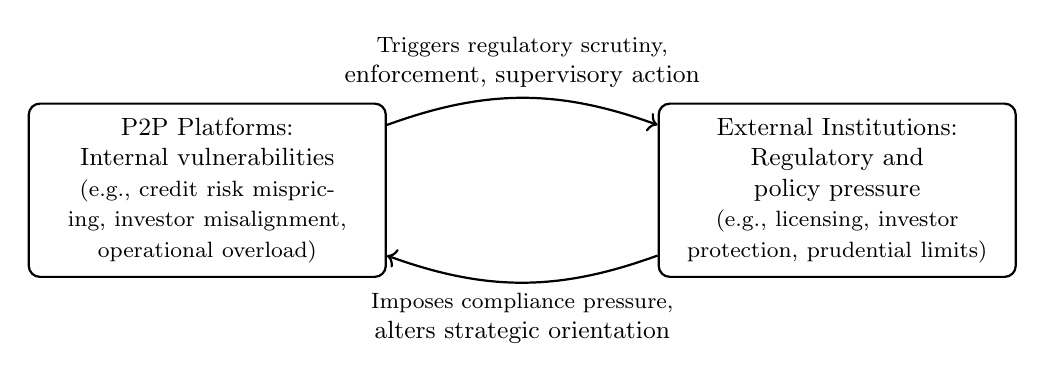
\begin{tikzpicture}[
        node distance=8cm,
        every node/.style={font=\small},
        box/.style={draw, rounded corners, thick, text width=4.3cm, align=center, minimum height=2.2cm}
        ]
        % Nodes
        \node[box] (A) {P2P Platforms:\\ Internal vulnerabilities\\ \footnotesize (e.g., credit risk mispricing, investor misalignment, operational overload)};
        \node[box, right of=A] (B) {External Institutions:\\ Regulatory and policy pressure\\ \footnotesize (e.g., licensing, investor protection, prudential limits)};

        % Arrows with bends
        \draw[->, thick, bend left=20] (A) to node[above, align=center] {\footnotesize Triggers regulatory scrutiny,\\ enforcement, supervisory action} (B);
        \draw[->, thick, bend left=20] (B) to node[below, align=center] {\footnotesize Imposes compliance pressure,\\ alters strategic orientation} (A);
    \end{tikzpicture}
    \caption{Dynamic feedback loop between internal platform vulnerabilities and regulatory responses}
    \label{fig:feedback_loop}
\end{figure}



\subsection{Diverging platform strategies and the erosion of the original P2P model}
Platform responses to these pressures varied by market structure, borrower profile, and strategic priorities. LendingClub and Zopa transitioned fully to banking models, while Prosper and Faircent retained simplified P2P features supported by automation and regulatory adaptation. These differences reflect variation in internal capacity to manage compliance, investor engagement, and product scalability.

Platforms with narrower borrower segments and streamlined risk models—such as Prosper—were better positioned to preserve basic P2P structures. Others, including Bondora and Faircent, shifted towards automated allocation systems that minimized investor discretion. Conversely, platforms pursuing broader service portfolios often found that the original P2P model created frictions with operational control and compliance efficiency.

As platforms grew, the burden of maintaining transparency and effective risk-sharing increased. While default risk formally remained with investors, the complexity of credit servicing and investor communication led to increased expectations that platforms assume implicit responsibility, thereby undermining the decentralized premise of P2P lending.

\subsection{Implications for platform evolution and policy design}
The evidence suggests that sustaining a retail-focused, investor-driven P2P model is increasingly difficult under conditions of regulatory maturity and market expansion. Platforms have either internalized risk through licensing and balance sheet lending or outsourced funding to institutional capital providers. 

For regulators, the findings highlight the need to design proportional and forward-looking oversight frameworks. Jurisdictions that imposed early supervisory structures—such as the UK and India—saw gradual formalization, whereas loosely regulated markets experienced rapid growth followed by abrupt collapse. These trajectories underscore the value of early-stage regulation aligned with long-term financial stability goals.

Overall, the transformation from P2P lending reflects a reconfiguration of financial intermediation models in response to both operational challenges and institutional expectations. As platforms evolve, the functional boundaries between FinTech platforms and traditional intermediaries continue to blur, raising new questions about how innovation can coexist with regulatory consistency and investor protection.

\section{Conclusion}\label{sec13}

This study addresses a novel research gap by integrating the analysis of platform-level risk structures with cross-national regulatory change to explain platform exit decisions. While existing literature has examined these aspects in isolation, our comparative approach highlights their joint influence on the structural transformation of the P2P lending sector.

This study examined the widespread transformation from P2P lending models by major global platforms. Through a comparative analysis of eight cases across multiple jurisdictions, we explored how internal operational limitations and external regulatory developments jointly influenced platform strategies.

The findings indicate that the original P2P model, based on decentralized risk allocation and retail participation, has become difficult to sustain as platforms mature and regulatory obligations intensify. In response, many platforms transitioned to hybrid or centralized structures that prioritize operational control, institutional capital, or full banking integration. \textcolor{NavyBlue}{This pattern suggests that decentralized financial intermediation, while initially disruptive, faces mounting pressures to institutionalize when scaled within formal regulatory systems. These insights may also hold implications for emerging decentralized finance (DeFi) ecosystems, which similarly rely on disintermediation but are only beginning to confront large-scale regulatory scrutiny.}

These developments reflect how FinTech models must evolve alongside regulatory environments and operational demands. Rather than viewing the retreat from P2P as a failure, it may be more accurate to interpret it as a shift toward institutional compatibility under conditions of market expansion and policy convergence. \textcolor{NavyBlue}{From a theoretical perspective, this study contributes to the understanding of platform evolution under institutional pressure. By linking internal fragilities to external rule changes, it moves beyond static categorizations of business models and highlights the adaptive dynamics of organizational restructuring. It also extends existing research on FinTech regulation by showing how platforms do not merely comply with regulatory change but actively reshape their strategic orientation in response. These insights contribute to broader debates on how digital financial intermediaries negotiate sustainability within increasingly formalized market environments.}

This study relied on publicly available platform and regulatory data, which may not capture informal supervisory interactions or unreported internal considerations. Further research could investigate platform governance structures, investor composition shifts, and funding model transitions using longitudinal methods and direct stakeholder engagement. Comparative work on decentralized finance and other FinTech lending models may also reveal whether similar pressures apply across different intermediation architectures. 

\textcolor{NavyBlue}{
Looking ahead, future research could extend this study along both substantive and methodological dimensions. Substantively, scholars may investigate the post-2024 trajectories of major P2P platforms—especially those that have adopted hybrid or institutional models—to assess whether their current configurations yield greater stability, regulatory acceptance, or market reach. Additionally, researchers could examine how different governance mechanisms, trust-building strategies, and investor engagement practices shape platform resilience in varied institutional environments. For instance, cross-national comparisons could further clarify why certain platforms exited the P2P model entirely while others persisted under modified structures. Methodologically, future work could complement our document-based analysis by incorporating interviews with platform executives, investors, and regulators, or by conducting in-depth case studies. Such approaches may uncover informal supervisory interactions, unreported operational challenges, or strategic considerations not reflected in public data. These techniques would help produce a more granular understanding of platform governance and transformation, thereby enhancing the explanatory depth of research on FinTech intermediation under institutional pressure.
}

Taken together, the results suggest that the long-term viability of disintermediated finance models depends not only on technological capacity but also on the ability to adapt to changing regulatory and operational conditions.

\newpage
\bibliography{references}% common bib file
%% if required, the content of .bbl file can be included here once bbl is generated
%%\input sn-article.bbl

\end{document}
